\section{Theoretischer Hintergrund}

\subsection{Fusee}

\begin{figure}[htbp]
  \centering
  \fbox{
    
\includegraphics[width=0.3\textwidth]{images/FuseeLogo375}
  }
  \caption{Fusee Logo}
  \label{fig:FuseeLogo}
\end{figure}

Die Furtwangen University Simulation and Entertainment Engine ist eine 3D-Grafik-Engine, die an der Fakultät Digitale Medien der Hochschule Furtwangen University seit dem Wintersemester 13/14 entwickelt wird. Fusee wird derzeit überwiegend von Studenten im Projektstudium, verschiedenen Wahlpflichtmodulen, Bachelor- sowie Master-Thesen weiter entwickelt. Fusee ist speziell für das Lernen und Lehren im Bereich der 3D-Grafik, Spiele und Simulationen gedacht und ermöglicht in dieser Hinsicht Zugriff auf tiefliegende Funktionen (vergleiche \cite{Muller.2014}).

Grundsätzlich versucht Fusee so viele Plattformen wie möglich zu bedienen. Hierunter zum Beispiel Windows, Linux, Android, iOS und auch HTML5/WebGL fähige Browser. Fusee verfolgt einen hoch modularen Ansatz, jegliche extern anprogrammierte Software und auch teilweise interne bereitgestellte Methoden sollen vom Benutzer der Engine ausgetauscht werden können. Beispiele für Module sind die Grafikanbindung von OpenGL über OpenTK oder die Physikanbindung von Bullet über BulletSharp (siehe \cite{Schey.2014}). Bisher bietet Fusee noch keine Implemtierung von Picking-Verfahren.

\begin{figure}[ht!]
  \centering
  \fbox{
    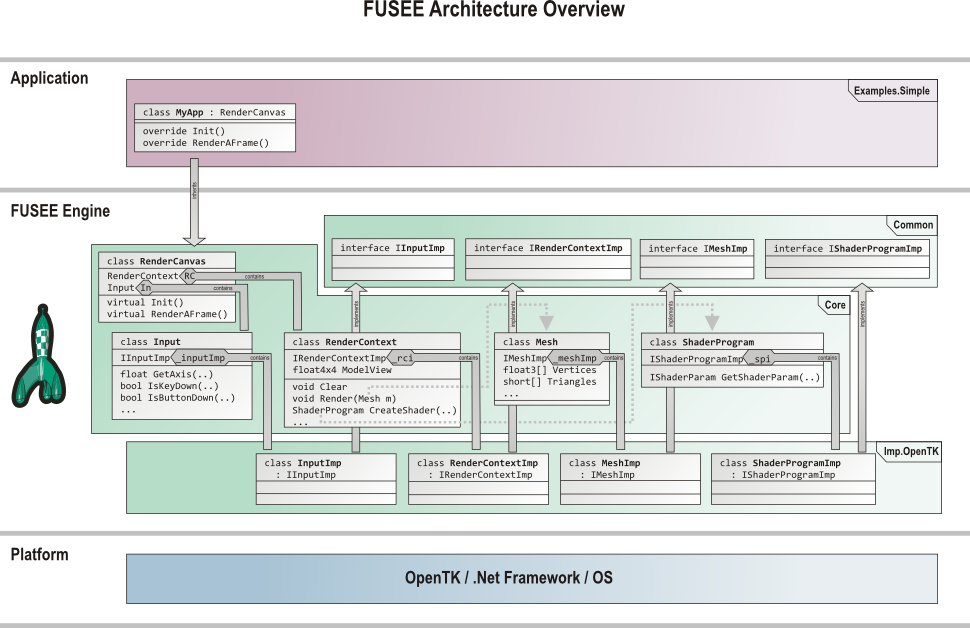
\includegraphics[width=1\textwidth]{images/FuseeArchitecture}
  }
  \caption{Fusee Aufbau}
  \label{fig:FuseeAufbau}
\end{figure}

Seinen modularen Aufbau erreicht Fusee dadurch, dass der Programmcode in drei Bereiche aufgeteilt wird. Der 'Core' beinhaltet alle grundlegenden internen Funktion, der 'Platform Adapter' beinhaltet die Anprogrammierung externen Codes und 'Common' stellt die Funktionalität der Implementierung über Interfaces bereit.

\subsection{Cinema 4D}

\subsection{Unity 3D}